
\documentclass{article}
\newenvironment{problem2}[1]{\noindent {\bf (#1}}
{\medskip}

\newenvironment{problem1}[1]{\noindent {\bf Problem #1:}}
{\medskip}
\usepackage{graphicx}
\usepackage{amsmath,amssymb,amsthm,amsfonts,graphicx,url,colordvi}
\usepackage{amssymb}
\usepackage{mathtools}
\usepackage[hyperfootnotes=false]{hyperref}
\usepackage{geometry}

\newcommand{\nat}{\mathbb{N}}
\newcommand{\real}{\mathbb{R}}
\newcommand{\realn}[1]{\mathbb{R}^{#1}}
\newcommand{\integer}{\mathbb{Z}}
\newcommand{\rational}{\mathbb{Q}}

\newcommand{\comp}[1]{#1^{\cal C}}
\newcommand{\ray}[1]{\overrightarrow{#1}}
\renewcommand{\line}[1]{\stackrel{\longleftrightarrow}{#1}}
\newcommand{\seg}[1]{\overline{#1}}
\renewcommand{\deg}{^{\circ}}

\newcommand{\forward}{\noindent ($\Longrightarrow$)}
\newcommand{\back}{\noindent ($\Longleftarrow$)}

\newcommand{\subst}{\noindent $(\subseteq)$\hspace{.1in}}
\newcommand{\supst}{\noindent $(\supseteq)$ \hspace{.1in}}

\title{Math 327: Final Take-home Solutions}
\author{by Sam Tay}
\date{\today}

\begin{document}

\begin{flushright}Sam Tay\\ Professor Schumacher \\ Math 230\\ Section 3.5: 1,4,6\\Section 3.2: 12(c)\\10/02/12\\\end{flushright}

\begin{problem1}{1} If $l\perp m$, then $l$ and $m$ contain rays that make four different right angles.
\end{problem1}
\begin{proof} Suppose $l\perp m$. By Definition 3.5.8, there is a point $A$ that lies on both $l$ and $m$, and $B\in l$, $D\in m$ such that rays $\ray{AD}$ and $\ray{AB}$ form a right angle $\angle{BAD}$. Next let $C\in l$ so that $C*A*B$ and $E\in m$ so that $E*A*D$. \\
\begin{center}
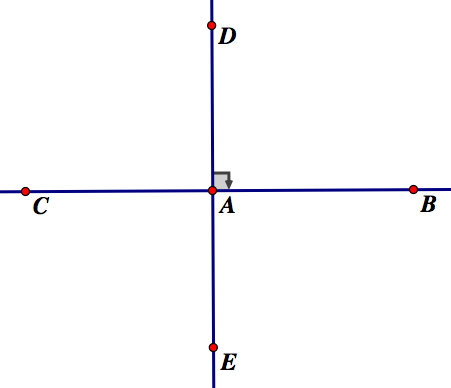
\includegraphics[width=2.5in]{S3_5_1.png}
\end{center}
Then of course, since $\ray{AC}$ and $\ray{AB}$ are opposite rays, $\angle{BAD}$ and $\angle{DAC}$ form a linear pair. By the Linear Pair Theorem, $$180\deg=\mu(\angle{BAD})+\mu(\angle{DAC})=90\deg+\mu(\angle{DAC}),$$ so $\mu(\angle{DAC})=90\deg$ and thus $\angle{DAC}$ is a right angle. Next we have opposite rays $\ray{AE}$ and $\ray{AD}$, so that $\angle{DAC}$ and $\angle{CAE}$ form a linear pair. Again by the Linear Pair Theorem, $$180\deg=\mu(\angle{DAC})+\mu(\angle{CAE})=90\deg+\mu(\angle{CAE}),$$ and similarly $\angle{CAE}$ is a right angle as well. Finally, the opposite rays $\ray{AC}$ and $\ray{AB}$ form the linear pair $\angle{CAE}$ and $\angle{EAB}$, so that $$180\deg=\mu(\angle{CAE})+\mu(\angle{EAB})=90\deg+\mu(\angle{EAB}),$$ so we have a fourth right angle $\angle{EAB}$.

To conclude that these are four distinct right angles, we will show that the four rays $\ray{AB},\ray{AD},\ray{AC},\ray{AE}$ are distinct. Our initial assumption is that $\mu(\angle{BAD})=90\deg\ne0\deg$, so $\ray{AB}\ne\ray{AD}$. Also since this angle is defined, $\ray{AB}$ and $\ray{AD}$ are nonopposite. We defined $C$ such that $\ray{AC}$ is opposite to $\ray{AB}$ and thus $\ray{AC}\ne\ray{AB}$ and $\ray{AC}\ne\ray{AD}.$ So the first three rays are distinct. Next, $E$ is defined such that $\ray{AE}$ is opposite to $\ray{AD}$, so $\ray{AE}\ne\ray{AD}$. Also $\ray{AE}\ne\ray{AC}$, otherwise $\ray{AE}$ would be opposite to $\ray{AB}$, implying $\ray{AD}=\ray{AB},$ which is not the case. Lastly, $\ray{AE}\ne\ray{AB},$ otherwise $\ray{AB}$ would be opposite to $\ray{AD}$, which we already said is not the case. Thus these four rays are distinct, and so are the four right angles they form.\end{proof}


\begin{problem1}{4} Supplements of congruent angles are congruent. \end{problem1}
\begin{proof} Let $\angle{ABC}\cong\angle{DEF}$, and suppose $\angle{XYZ}$ is a supplement to $\angle{ABC}$ and $\angle{UVW}$ is a supplement to $\angle{DEF}$. From this assumption of supplements we have $$\mu(\angle{ABC})+\mu(\angle{XYZ})=180\deg$$ $$\mu(\angle{DEF})+\mu(\angle{UVW})=180\deg,$$ so that $$\mu(\angle{XYZ})=180\deg-\mu(\angle{ABC})$$ $$\mu(\angle{UVW})=180\deg-\mu(\angle{DEF}).$$ However the congruence above implies that $\mu(\angle{ABC})=\mu(\angle{DEF}),$ and it follows immediately that $\mu(\angle{XYZ})=\mu(\angle{UVW})$, and therefore supplements of congruent angles are also congruent.
\end{proof}


\begin{problem1}{6} If $A,B,C,D,$ and $E$ are points such that $A*B*C$, $D$ and $E$ are on opposite sides of $\line{AB}$, and $\angle{DBC}\cong\angle{ABE},$ then $D, B,$ and $E$ are collinear. \end{problem1}
\begin{proof} As above, suppose $A,B,C,D,$ and $E$ are points such that $A*B*C$, $D$ and $E$ are on opposite sides of $\line{AB}$, and $\angle{DBC}\cong\angle{ABE}.$ 
\begin{center}
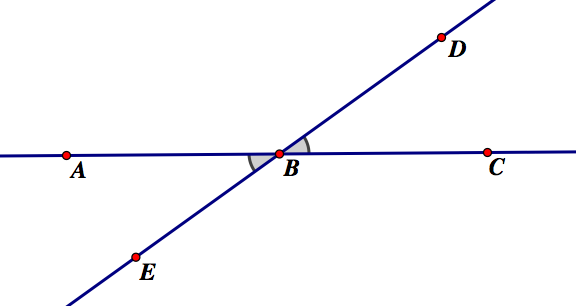
\includegraphics[width=3.7in]{S3_5_6.png}
\end{center} We will first show that $A$ and $C$ are on opposite sides of the line $\line{BE}$. Since $E$ and $D$ are defined to be on opposite sides of $\line{BA}$, we know that $E\notin\line{BA}$, where $\line{BA}=\line{AC}$, so $\line{BE}\ne\line{AC}$. But $\{B\}\subseteq\line{BE}\cap\line{AC}$, so these lines are distinct and nonparallel. By Theorem 3.1.7 we know that $B$ is the only point that lies on both $\line{BE}$ and $\line{AC}$. Hence $A,C\notin\line{BE}$ and, since $A*B*C$, we have $\{B\}\subseteq\line{BE}\cap\seg{AC}$. By Proposition 3.3.4, we know $A$ and $C$ are on opposite sides of $\line{BE}$ and can define the two distinct half-planes $H_A$ and $H_C$ that are bounded by $\line{BE}$.

To show that $D\in\line{BE}$, suppose instead that $D\notin\line{BE}$. Then we have two cases\footnote{I think I can suppose without loss of generality that $D\in H_A$, but I'll just present both arguments to be on the safe side.}: either $D\in H_A$ or $D\in H_C$. If $D\in H_A$, then $D$ and $A$ are on the same side of $\line{BE}$. 
\begin{center}
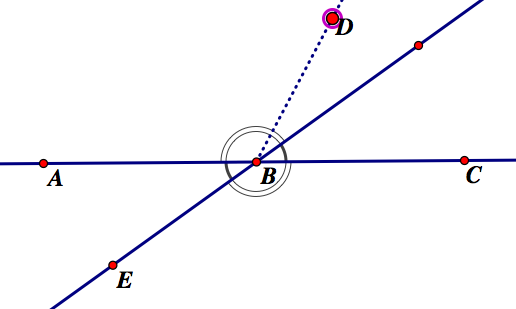
\includegraphics[width=3.5in]{S3_5_6b.png}
\end{center}
Since $A*B*C$, the external point $D$ forms the linear pair $\angle{ABD}$ and $\angle{DBC}$. By the Linear Pair Theorem, we have
\begin{align*}
180\deg&=\mu(\angle{ABD} )+\mu(\angle{DBC})\\
&=\mu(\angle{ABD} )+\mu(\angle{ABE}),
\end{align*} so $\angle{ABD}$ and $\angle{ABE}$ are supplementary as well. Note that since $\mu(\angle{ABE} )<180\deg,$ we have $\angle{ABD}\ne0\deg$, so that $D$ does not lie on $\ray{BA}$. Therefore we can apply Theorem 3.4.4 to conclude that either $D$ is in the interior of $\angle{EBA}$ or $A$ is in the interior of $\angle{EBD}$. However, $D$ cannot be in the interior of $\angle{EBA}$, because this would require $D$ and $E$ on the same side of $\line{AB}$, which contradicts our original hypothesis. So it must be the case that $A$ is in the interior of $\angle{EBD}$, and the Angle Addition Postulate implies that
\begin{align*} \mu(\angle{EBD})&=\mu(\angle{EBA})+\mu(\angle{ABD})\\
&=\mu(\angle{ABE})+\mu(\angle{ABD})=180\deg.
\end{align*} 
This of course is a contradiction, as $180\deg$ is not in the range of $\mu$. (Our false assumption of $D\in H_A$ implies that rays $\ray{BE},\ray{BD}$ are nonopposite, allowing $\angle{EBD}$ to be defined.)

Next suppose that $D\in H_C$. Then $D$ and $C$ are on the same side of $\line{BE}$.
\begin{center}
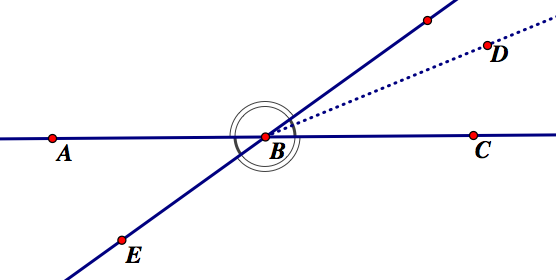
\includegraphics[width=3.5in]{S3_5_6c.png}
\end{center}
Since $A*B*C$, the external point $E$ forms the linear pair $\angle{ABE}$ and $\angle{EBC}$. By the Linear Pair Theorem, we have
\begin{align*}
180\deg&=\mu(\angle{ABE} )+\mu(\angle{EBC})\\
&=\mu(\angle{DBC} )+\mu(\angle{EBC}),
\end{align*} 
 so $\angle{DBC}$ and $\angle{EBC}$ are supplementary as well. Note that since $\mu(\angle{EBC} )<180\deg,$ we have $\angle{DBC}\ne0\deg$, so that $D$ does not lie on $\ray{BC}$. Then again by Theorem 3.4.4, we know that either $D$ is in the interior of $\angle{EBC}$ or $C$ is in the interior of $\angle{EBD}$. However, since $E$ and $D$ are defined to be on opposite sides of $\line{AB}=\line{BC}$, we cannot have $D$ in the interior of $\angle{EBC}$. Thus it must be the case that $C$ is in the interior of $\angle{EBD}$. Then by the Angle Addition Postulate, \begin{align*} \mu(\angle{EBD})&=\mu(\angle{EBC})+\mu(\angle{CBD})\\
 &=\mu(\angle{EBC})+\mu(\angle{DBC})=180\deg.\end{align*}
 We find the same contradiction in either case, and conclude that $D$ is not in either of the half-planes bounded by $\line{BE}$. Of course, this means that $D\in\line{BE}$, so that $E,B$, and $D$ are collinear.
\end{proof}

\begin{problem1}{3.2.12(c)} If $f:\ell\to\real$ is a coordinate function for a line $\ell$ and $h:\ell\to\real$ is another coordinate function for $\ell$, then there exists a constant $c$ such that either $h(R)=f(R)+c$ or $h(R)=-f(R)+c.$
\end{problem1}

\begin{proof} Since $f$ is a coordinate function there exist $P,Q \in\ell$ such that $f(P)=0$ and $f(Q)=1$. We know $P$ and $Q$ are distinct because $f$ is well-defined, and since $h$ is injective, the law of trichotomy in $\real$ gives two possibilities: $h(P)<h(Q)$ or $h(Q)<h(P).$ Let $c=h(P).$ If $h(P)<h(Q)$, we will show that $h(R)=f(R)+c$. First we verify this for the points $P$ and $Q$. We have $$h(P)=0+h(P)=f(P)+c,$$ and since coordinate functions preserve distance, we find 
 \begin{align*} QP&= |f(Q)-f(P)| =|f(Q)-0|= f(Q) \\
  &= |h(Q)-h(P)| =h(Q)-h(P)=h(Q)-c.\end{align*} The penultimate equality follows because $h(P)<h(Q)$. Of course from these equations, we have $h(Q)=f(Q)+c.$ Next, suppose $R*P*Q$. Then by Theorem 3.2.17, we have $f(R)<f(P)<f(Q)$ and $h(R)<h(P)<h(Q)$ and therefore\begin{align*} RP &=  |f(R)-f(P)| = f(P)-f(R) = -f(R) \\
  &=|h(R)-h(P)| = h(P)-h(R) = c - h(R). \end{align*} Therefore $h(R)=f(R)+c$. Next we suppose $P*R*Q$. Then again by Theorem 3.2.17, we have $f(P)<f(R)<f(Q)$ and $h(P)<h(R)<h(Q).$ Then
  \begin{align*} RP &=  |f(R)-f(P)| = f(R)-f(P) = f(R) \\
  &=|h(R)-h(P)| = h(R)-h(P) = h(R)-c. \end{align*} Again we find $h(R)=f(R)+c.$ Finally, suppose $P*Q*R$, so that $f(P)<f(Q)<f(R)$ and $h(P)<f(Q)<f(R)$. Again we have   \begin{align*} RP &=  |f(R)-f(P)| = f(R)-f(P) = f(R) \\
  &=|h(R)-h(P)| = h(R)-h(P) = h(R)-c, \end{align*} identical to the previous case. We have shown now that if $h(P)<h(Q)$, then for any $R\in\ell$, $h(R)=f(R)+c$.
  
  Next suppose $h(Q)<h(P)$, in which case we will show that $h(R)=-f(R)+c$. First we verify this for the points $P$ and $Q$. We have $$h(P)=-0+h(P)=-f(P)+c,$$ and 
  \begin{align*} QP&= |f(Q)-f(P)| =|f(Q)-0|= f(Q) \\
  &= |h(Q)-h(P)| =h(P)-h(Q)=-h(Q)+c,\end{align*}  from which it follows that $h(Q)=-f(Q)+c$. Next suppose $R*P*Q$, so that $f(R)<f(P)<f(Q)$ and $h(Q)<h(P)<h(R).$ Then
  \begin{align*} RP &=  |f(R)-f(P)| = f(P)-f(R) = -f(R) \\
  &=|h(R)-h(P)| = h(R)-h(P) =  h(R)-c, \end{align*}  so $h(R)=-f(R)+c$. If $P*R*Q$, then $f(P)<f(R)<f(Q)$ and $h(Q)<h(R)<h(P),$ and 
  \begin{align*} RP &=  |f(R)-f(P)| = f(R)-f(P) = f(R) \\
  &=|h(R)-h(P)| = h(P)-h(R) =  -h(R)+c.\end{align*} Again it follows that $h(R)=-f(R)+c$. Lastly, if $P*Q*R$, then $f(P)<f(Q)<f(R)$ and $h(R)<h(Q)<h(P),$ and
  \begin{align*} RP &=  |f(R)-f(P)| = f(R)-f(P) = f(R) \\
  &=|h(R)-h(P)| = h(P)-h(R) = -h(R)+c. \end{align*} Again we find $h(R)=-f(R)+c$. This shows that if $h(Q)<h(P)$, then for any $R\in\ell$, we have $h(R)=-f(R)+c$. We conclude that for any two coordinate functions $f,h$ for a line $\ell$, there is a constant $c$ such that $h(R)=f(R)+c$ or $h(R)=-f(R)+c.$

\end{proof}




\end{document}



Otherwise, suppose $\mu(\angle{DBC})=\mu(\angle{ABE})>0\deg.$ We will first show that $A$ and $C$ are on opposite sides of the line $\line{BE}$. Since $E$ and $D$ are defined to be on opposite sides of $\line{BA}$, we know that $E\notin\line{BA}$, where $\line{BA}=\line{AC}$, so $\line{BE}\ne\line{AC}$. But $\{B\}\subseteq\line{BE}\cap\line{AC}$, so these lines are distinct and nonparallel. By Theorem 3.1.7 we know that $B$ is the only point that lies on both $\line{BE}$ and $\line{AC}$. Hence $A,C\notin\line{BE}$ and, since $A*B*C$, we have $\{B\}\subseteq\line{BE}\cap\seg{AC}$. By Proposition 3.3.4, we know $A$ and $C$ are on opposite sides of $\line{BE}$ and can define the two distinct half-planes $H_A$ and $H_C$ that are bounded by $\line{BE}$.



we are assuming $\mu(\angle{ABE})>0\deg$, we know that rays $\ray{BA},\ray{BE}$ are distinct and nonopposite. Hence $\line{BE}\ne\line{BA}$, so $\line{BE}\ne\line{AC}$. Therefore by Exercise 3.2.1, we know that $B$ is the only point that lies on both $\line{BE}$ and $\line{AC}$, and since 


 First we will prove a trivial case: if $\mu(\angle{DBC})=\mu(\angle{ABE})=0\deg,$ then $\ray{BD}=\ray{BC}$ and $\ray{BA}=\ray{BE}$. From this it follows immediately that $\line{BD}=\line{BC}$ and $\line{BA}=\line{BE}$. Since $A*B*C$, we have $\line{BC}=\line{BA}$, and this would imply $\line{BD}=\line{BE}$, so that $E,B,$ and $D$ are collinear.

Otherwise, suppose $\mu(\angle{DBC})=\mu(\angle{ABE})>0\deg.$ 





